\section{Task3: Architecture design}
\subsection{Architectural diagram}

\newpage
\subsection{Component Diagram}
\textbf{Student Client subsystem}
\begin{itemize}
    \item \textbf{Login component}: Cho phép sinh viên đăng nhập vào hệ thống bằng cách giao tiếp với \textbf{Authenticate} để xác thực.
    \item \textbf{Print component}: Cho phép sinh viên bắt đầu quá trình in. Bao gồm việc tải tệp lên, chọn máy in và cài đặt in và xác nhận lệnh in.
    \item \textbf{BuyPrintingPages component}: Cho phép sinh viên mua thêm các trang in nếu cần trước khi in. Tương tác với server để bắt đầu quá trình thanh toán.
\end{itemize}

\textbf{Server subsystem}
\begin{itemize}
    \item \textbf{Authenticate component}: Xử lý xác thực người dùng bằng cách giao tiếp với \textbf{HCMUT\_SSO} để xác minh danh tính sinh viên.
    \item \textbf{ProfileController component}: Quản lý thông tin hồ sơ sinh viên, truy xuất dữ liệu từ \textbf{Database} khi cần.
    \item \textbf{PrintController component}: Xử lý các yêu cầu in từ client, bao gồm kiểm tra số trang có sẵn và gửi lệnh in tới máy in đã chọn.
    \item \textbf{LogsController component}: Ghi nhận và quản lý nhật ký in ấn để theo dõi, tương tác với \textbf{Database} để lưu trữ thông tin này.
    \item \textbf{BuyController component}: Quản lý việc mua thêm các trang in thông qua tương tác với \textbf{BKPay} để xử lý thanh toán.
\end{itemize}

\textbf{Dịch vụ Bên ngoài}
\begin{itemize}
    \item \textbf{HCMUT\_SSO}: Cung cấp xác thực Single Sign-On (SSO), cho phép sinh viên truy cập tài khoản một cách an toàn.
    \item \textbf{Database}: Lưu trữ dữ liệu sinh viên, lịch sử in ấn, số trang có sẵn và các tài liệu đã tải lên.
    \item \textbf{Printer}: Thực hiện công việc in khi được \textbf{PrintController} ủy quyền.
    \item \textbf{BKPay}: Xử lý thanh toán cho các trang in bổ sung, xác nhận giao dịch thành công hoặc thất bại với server.
\end{itemize}
\newpage
\begin{figure}[htbp]
    \centering
    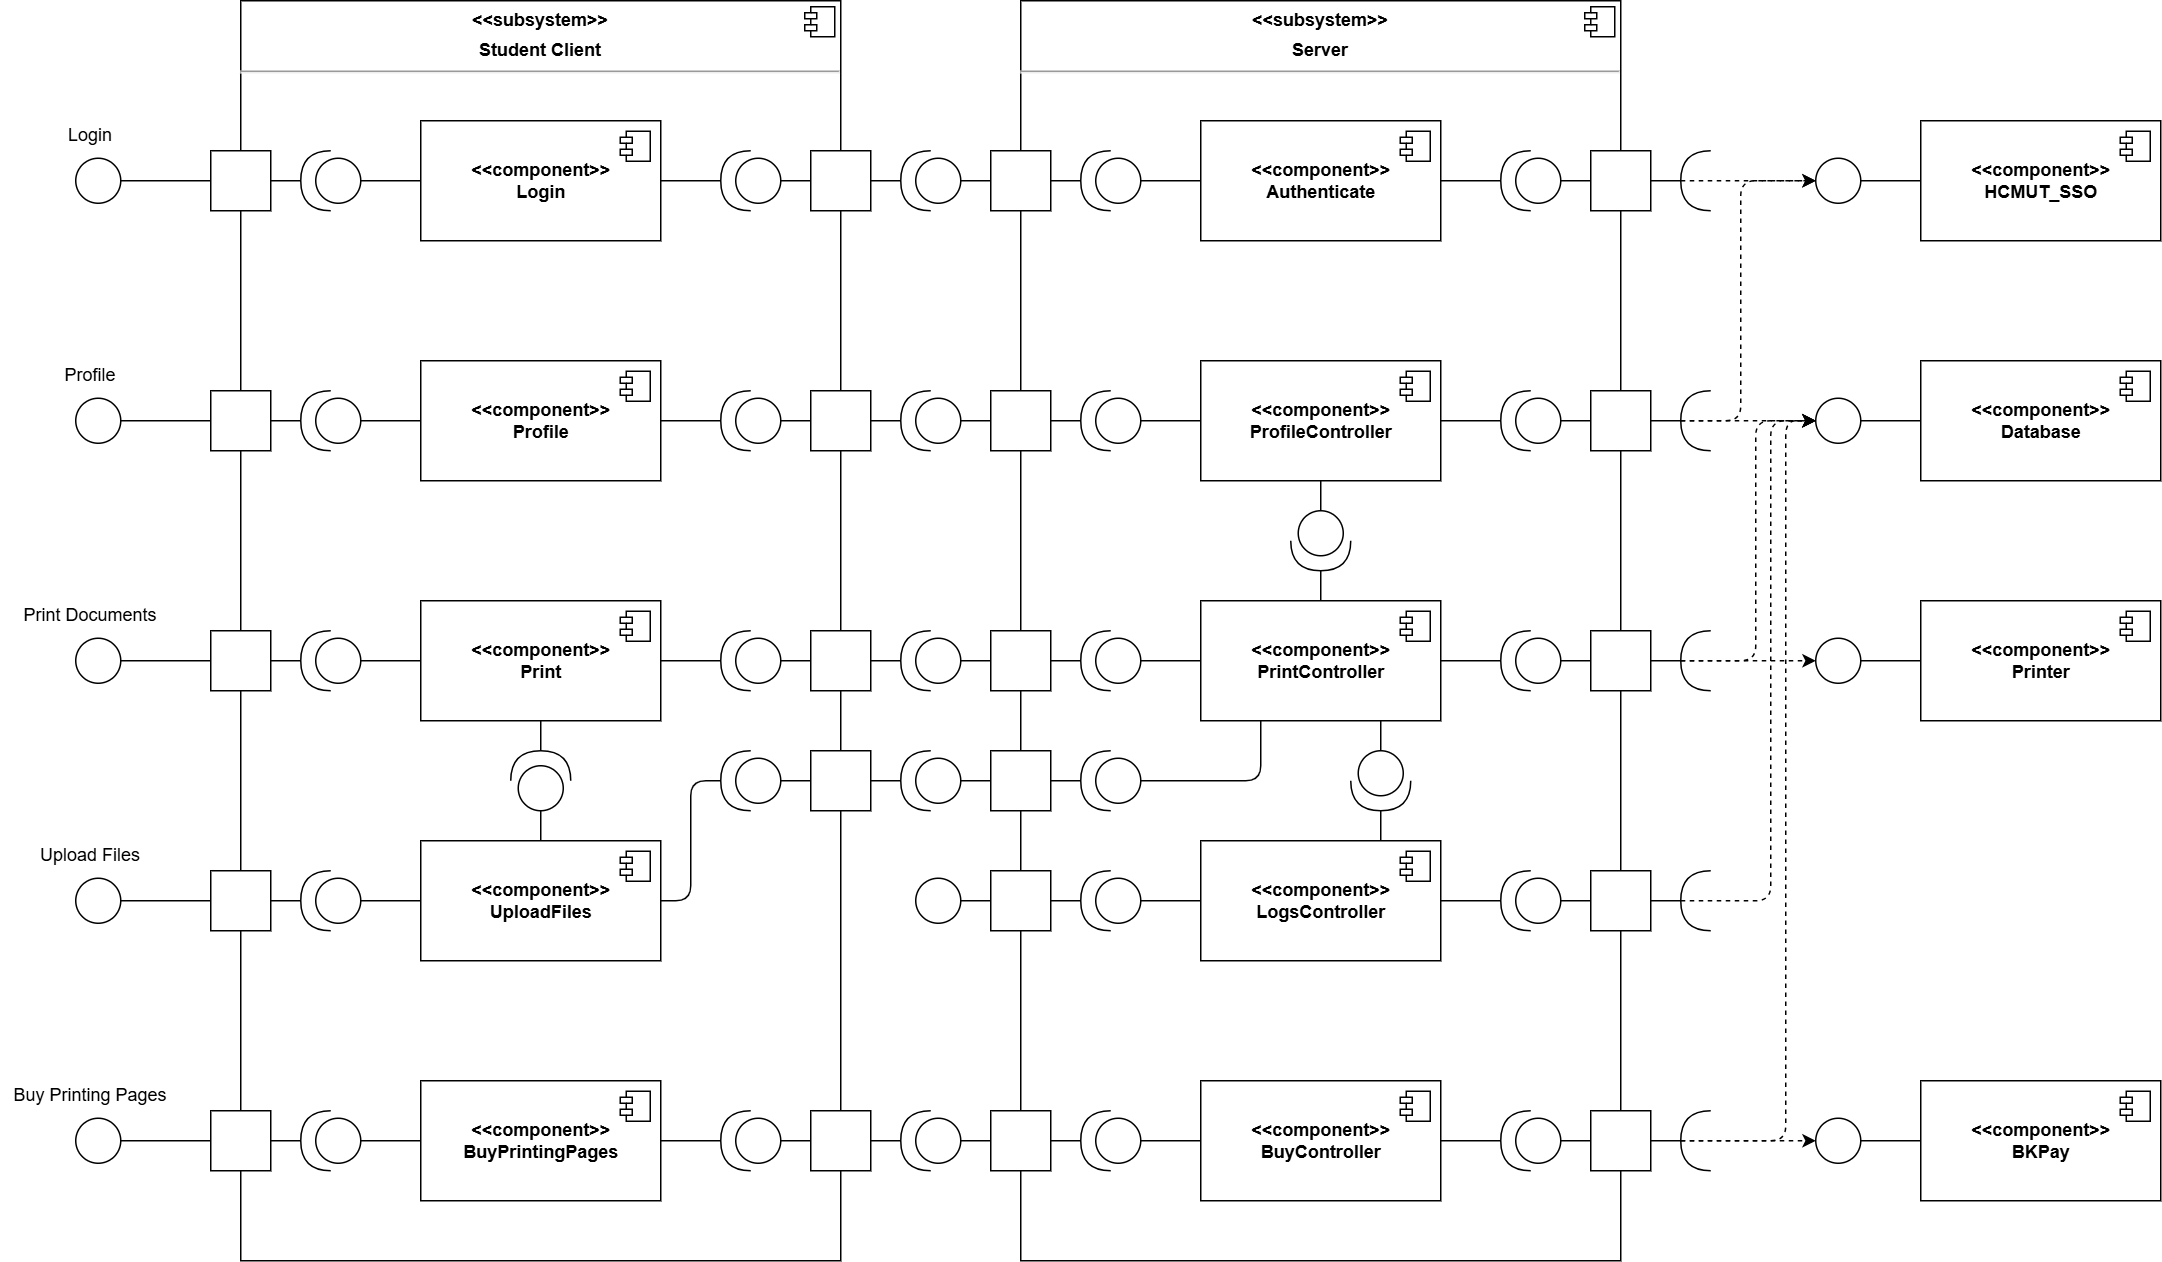
\includegraphics[width=1\linewidth]{Images/Diagrams/Print_component.png}
    \caption{Component Diagram}
\end{figure}
